\section{Three-Region Test Problem}

In this section, results are presented for the 3-region test
problem described in Section \ref{sec:three_region}.
Figure \ref{fig:three_region} compares the solutions computed
for each scheme for this problem, and
Table \ref{tab:three_region_run_parameters} shows the run parameters used.
%-------------------------------------------------------------------------------
\begin{table}[h]\caption{Three-Region Test Problem Run Parameters}
\label{tab:three_region_run_parameters}
\centering
\begin{tabular}{l l}\toprule
\emph{Parameter} & \emph{Value}\\\midrule
Number of Cells & $N_{cell} = 2^5 = 32$\\
End Time & $t = 1$\\
CFL Number & $\nu = 0.5$\\
Time Integrator & SSPRK33\\\midrule
Entropy Function & $E(u) = \frac{1}{2}u^2$\\
Entropy Residual Coefficient & $c_E = 0.1$\\
Entropy Jump Coefficient & $c_J = 0.1$\\
Entropy Time Integrator & BE\\
\bottomrule\end{tabular}
\end{table}
%-------------------------------------------------------------------------------
\begin{figure}[h]
   \centering
   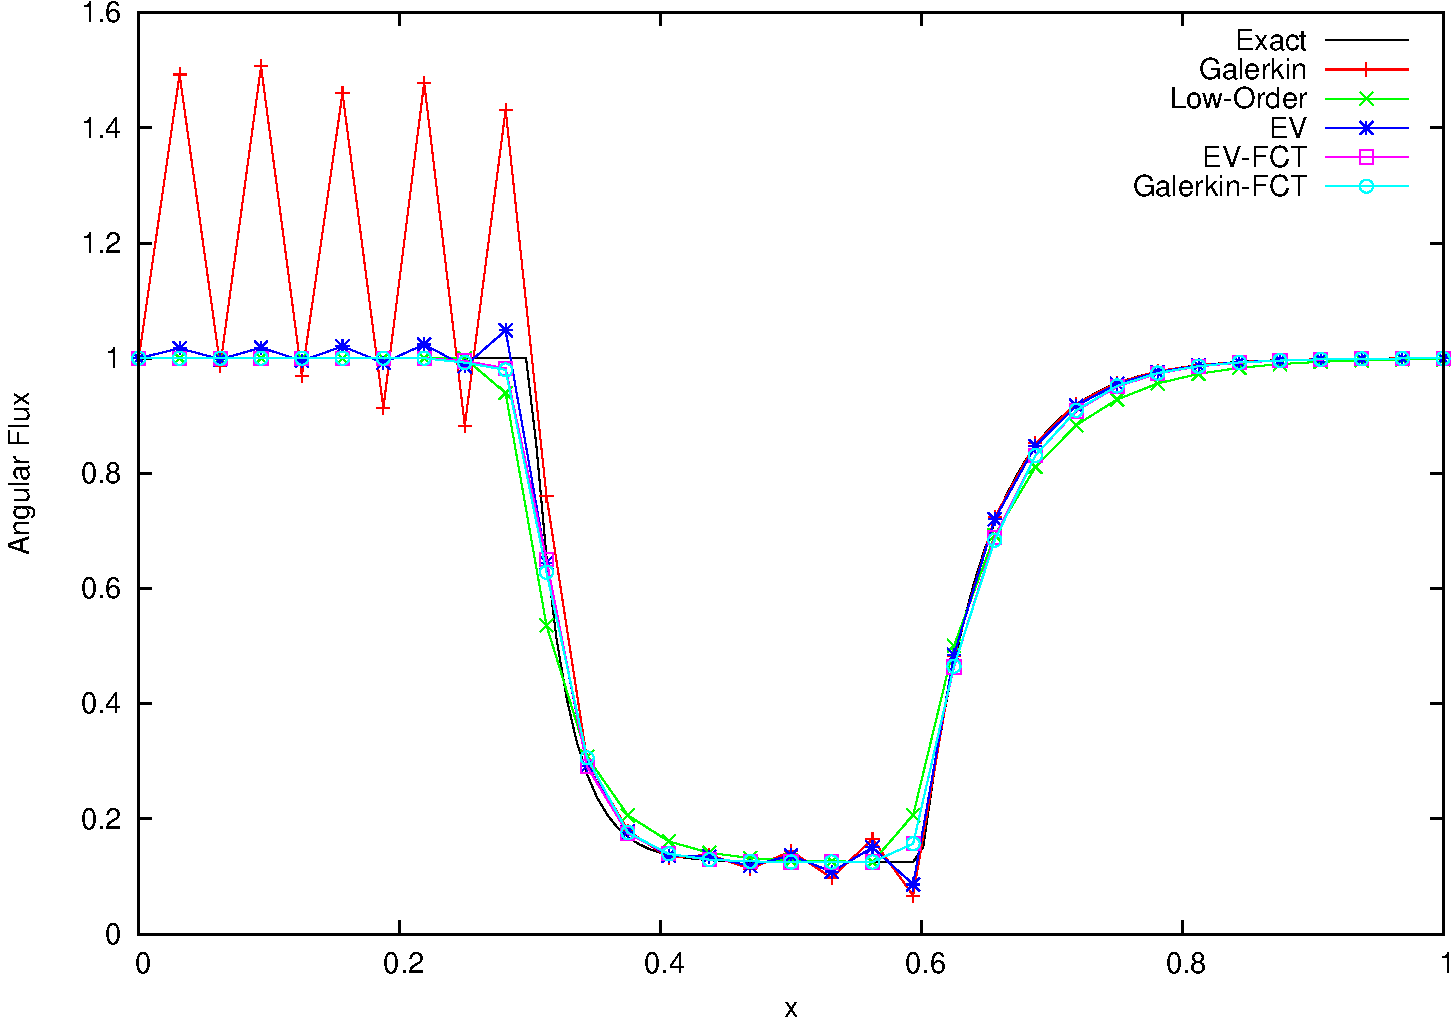
\includegraphics[width=0.9\textwidth]{three_region/three_region.pdf}
   \caption{Comparison of Solutions for the 3-Region Test Problem}
   \label{fig:three_region}
\end{figure}
%-------------------------------------------------------------------------------
\subsection{Code and Version}
Deal.ii code, git commit hash 0fe7871c020c606cef1734f03e653d49938f35bc
